\documentclass[tikz, convert={outext=.svg, command=\unexpanded{pdf2svg \infile\space\outfile}}, multi=false]{standalone}

\usepackage{tikz}
\usetikzlibrary{decorations}
\usetikzlibrary{decorations.pathmorphing}
\usetikzlibrary{decorations.pathreplacing}
\usetikzlibrary{decorations.shapes}
\usetikzlibrary{decorations.text}
\usetikzlibrary{decorations.markings}
\usetikzlibrary{decorations.fractals}
\usetikzlibrary{decorations.footprints}



\begin{document}

% \begin{tikzpicture}
%  \tikzstyle{every node}=[shape= circle,draw,text=red, thin];
%  \path
%  (2*0.766044,2*0.642788) node(3){3}
%  (2*0.173648,2*0.984808) node(4){4}
%  (2*-0.5,2*0.866025) node(5){5}
%  (2*-0.939693,2*0.34202) node(6){6}
%  (2*-0.939693,2*-0.34202) node(7){7}
%  (2*-0.5,2*-0.866025) node(8){8}
%  (2*0.173648,2*-0.984808) node(9){9}
%  (2*0.766044,2*-0.642788) node(1){1}
%  (2*1,0) node(2){2};
%
%  \draw [draw=blue, thick]
%  (9)--(3)--(1)--(5);
%  \draw [draw=orange,thick]
%  (8)--(4)--(2)--(6);
%  \draw [dashed]
%  (1)--(2)--(8)
%  (7)--(1)--(8)
%  (3)--(6)--(1)--(9)
%  (1)--(4)
%  ;
% \end{tikzpicture}



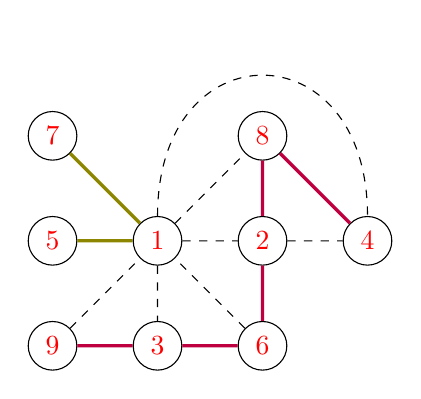
\begin{tikzpicture}
 \tikzstyle{every node}=[shape= circle,draw,text=red, thin];
 \path
 (0,0) node(9){9}
 (2*2/3,0) node(3){3}
 (4*2/3,0) node(6){6}
 (0,2*2/3) node(5){5}
 (2*2/3,2*2/3) node(1){1}
 (4*2/3,2*2/3) node(2){2}
 (6*2/3,2*2/3) node(4){4}
 (0,4*2/3) node(7){7}
 (4*2/3,4*2/3) node(8){8};

 \draw [draw=purple,very thick]
 (9)--(3)--(6)--(2)--(8)--(4);
 \draw [draw=olive, very thick]
 (7)--(1)--(5);
 \draw [dashed]
 (1)--(2)
 (9)--(1)--(3)
 (2)--(4)
 (6)--(1)--(8)
 ;
 \draw [dashed] (1) .. controls +(up:27mm) and +(up:27mm) .. (4);
\end{tikzpicture}

\end{document}
